
\section{Notation}
\label{section:notation}

\marginnote{Maybe you are feeling that this formality is unnecessary,
  or even ridiculous; why can't we just list off a few terms and pick
  up on the pattern intuitively?  As we'll see later, that might be
  very hard---nay, impossible---to do!  There might be very
  different---but equally reasonable---patterns that start the same
  way.

  To resolve this ambiguity, it is perhaps not so ridiculous to
  introduce the formalism of ``functions.''  Functions provide a nice
  language for associating numbers (terms) to other numbers
  (indices).}

\nobreak A ``sequence'' of numbers is just a list of numbers.  For
example, here is a list of numbers:
$$
1,\quad 1,\quad 2,\quad 3,\quad 5,\quad 8,\quad 13,\quad 21,\quad \ldots
$$
Note that numbers in the list can repeat.  And consider those little
dots at the end!  The dots ``\ldots'' signify that the list keeps
going, and going, and going---forever.  Presumably the sequence
continues by following the pattern that the first few ``terms''
suggest.  But what's that pattern?

To make this talk of ``patterns'' less ambiguous, it is useful to
think of a sequence as a function. We have up until now dealt with
functions whose domains are the real numbers, or a subset of the real
numbers, like $f(x)=\sin (1/x)$.

A real-valued function with domain the natural numbers
$\N=\{1,2,3,\ldots\}$ is a \defnword{sequence}.

Other functions will also be regarded as sequences: the domain might
include $0$ alongside the positive integers, meaning that the
domain is the non-negative integers, $\ds
\Z^{\ge0}=\{0,1,2,3,\ldots\}$.  The range of the function is still
allowed to be the real numbers; in symbols, the function $f\colon
\N\to\R$ is a sequence.


Sequences are written down in a few different, but equivalent,
ways; you might see a sequence written as
\begin{align*}
  & a_1,\quad a_2, \quad a_3, \quad\ldots, \\
  & a_n \\
  & \left(a_n\right)_{n \in \N}, \\
  & \left\{a_n\right\}_{n=1}^\infty, \\
  & \left\{f(n)\right\}_{n=1}^\infty, \quad \mbox{or} \\
  & \left(f(n)\right)_{n \in \N},
\end{align*}
depending on which author you read.  Worse, depending on the
situation, the same author (and this author) might use various
notations for a sequence!  In this textbook, I will usually write
$(a_n)$ if I want to speak of the sequence as a whole (think
\textit{gestalt}) and I will write $a_n$ if I am speaking of a
specific term in the sequence.

Let's summarize the preceding discussion in the following definition.
\begin{definition} \relax\index{sequence} A \defnword{sequence}
  $(a_n)$ is, formally speaking, a real-valued function with domain
  \[
  \{ n \in \Z : n \geq N \},\quad \mbox{for some integer $N$.}
  \]
  Stated more humbly, a sequence assigns a real number to the
  integers starting with an index $N$.

  The ``outputs'' of a sequence are the \defnword{terms} of the
  sequence; the ``$n^{\nth}$ term'' is the real number that the
  sequence associates to the natural number $n$, and is usually
  written $a_n$. \index{sequence!term} The $n$ in the phrase
  ``$n^{\nth}$ term'' is called an
  \defnword{index}\index{sequence!index}; the plural of index is
  either indices or indexes, depending on who you ask.  The first
  index $N$ is called the \defnword{initial
    index}\index{sequence!index!initial}.
\end{definition} 

\marginnote{Recall that the natural numbers $\N$ are the counting
  numbers $1, 2, 3, 4, \ldots$.  If we want our sequence to start at
  zero, we use $\Z^{\ge 0}$ as the domain instead.  The fancy symbols
  $\Z^{\ge 0}$ refer to the non-negative integers, which include zero
  (since zero is neither positive nor negative) and also positive
  integers (since they certainly aren't negative).}

\marginnote{To confuse matters further, some people---especially
  computer scientists---might include zero in the natural numbers
  $\N$.  Mathematics is cultural.}

\begin{warning}
  Usually the ``domain'' of a sequence is $\N$ and $\Z^{\ge 0}$.  But
  depending on the context, it may be convenient for a sequence to
  start somewhere else---perhaps with some negative number.  We
  shouldn't let the usual situation of $\N$ or $\Z^{\ge 0}$ get in the
  way of making the best choice for the problem at hand.
\end{warning}

As you can tell, there is a deep tension between precise definition
and a vague flexibility; as instructors, how we navigate that tension
will be a big part of whether we are successful in teaching the
course.  We need to invoke precision when we're tempted to be too
vague, and we need to reach for an extra helping of vagueness when the
formalism is getting in the way of our understanding.  It can be a
tough balance.

\section{Defining sequences}
\label{section:defining-sequences}

\subsection{Defining sequences by giving a rule}

Just as with functions with domain the real numbers, we will most
often encounter sequences that can be expressed by a formula.  In the
Introduction to this textbook, we saw the sequence given by the rule $\ds
a_i=f(i)=1-1/2^i$.  Other examples are easy to cook up, like
\begin{align*}
  a_i &={i\over i+1}, \\
  b_n &={1\over2^n}, \\
  c_n &=\sin(n\pi/6), \mbox{ or} \\
  d_i &={(i-1)(i+2)\over2^i}. \\
\end{align*}
Frequently these formulas will make sense if thought of either as
functions with domain $\R$ or $\N$, though occasionally the given
formula will make sense only for integers.  We'll address the
idea of a real-valued function ``filling in'' the gaps between the
terms of a sequence when we look at graphs in
Section~\xrefn{section:graphs}.

\begin{warning}
  A common misconception is to confuse the sequence with the rule for
  generating the sequence.  The sequences $(a_n)$ and $(b_n)$ given by
  the rules $a_n = (-1)^n$ and $b_n = \cos (\pi \, n)$ are, despite
  appearances, different rules which give rise to the \textit{same}
  sequence.  These are just different names for the same object.
\end{warning}

Let's give a precise definition for ``the same'' when speaking of sequences.

\marginnote{Compare this to equality for functions: two functions are
  the same if they have same domain and codomain, and they assign the
  same value to each point in the domain.}

\begin{definition}
  Suppose $(a_n)$ and $(b_n)$ are sequences starting at $1$.  These
  sequences are \defnword{equal}\index{sequence!equality} if for all
  natural numbers $n$, we have $a_n = b_n$.

  More generally, two sequences $(a_n)$ and $(b_n)$ are
  \defnword{equal} if they have the same initial index $N$, and for
  every integer $n \geq N$, the $n^{\nth}$ terms have the same value, that is,
  \[
  a_n = b_n \quad \mbox{for all $n \geq N$.}
  \]
\end{definition}
In other words, sequences are the same if they have the same set of
valid indexes, and produce the same real numbers for each of those
indexes---regardless of whether the given ``rules'' or procedures for
computing those sequences resemble each other in any way.

\subsection{Defining sequences using previous terms}

\marginnote{You might be familiar with \textit{recursion} from a
  computer science course.}

Another way to define a sequence is \textit{recursively}, that is, by
defining the later outputs in terms of previous outputs.  We start by
defining the first few terms of the sequence, and then describe how
later terms are computed in terms of previous terms.

\begin{example}
Define a sequence recursively by
$$
a_1 = 1, \quad a_2 = 3, \quad a_3 = 10,
$$
and the rule that $a_n = a_{n-1} - a_{n-3}$.  Compute $a_5$.
\end{example}

\begin{solution}
  First we compute $a_4$.  Substituting $4$ for $n$ in the rule $a_n = a_{n-1} - a_{n-3}$, we find
$$
a_4 = a_{4-1} - a_{4-3} = a_3 - a_1.
$$
But we have values for $a_3$ and $a_1$, namely $10$ and $1$, respectively.  Therefore $a_4 = 10 - 1 = 9$.

Now we are in a position to compute $a_5$.  Substituting $5$ for $n$ in the rule $a_n = a_{n-1} - a_{n-3}$, we find
$$
a_5 = a_{5-1} - a_{5-3} = a_4 - a_2.
$$
We just computed $a_4 = 9$; we were given $a_2 = 3$.  Therefore $a_5 = 9 - 3 = 6$.
\end{solution}

\marginnote{You can imagine some very complicated sequences defined recursively.  Make up your own sequence and share it with your friends!  Use the \href{https://twitter.com/search?q=\%23sequence}{hashtag \texttt{\#sequence}}.}


\section{Examples}
\label{section:examples}

\marginnote{Tons of entertaining sequences are listed in the \href{http://oeis.org/}{The On-Line Encyclopedia of Integer Sequences}.}

Mathematics proceeds, in part, by finding precise statements for
everyday concepts.  We have already done this for sequences when we
found a precise definition (``function from $\N$ to $\R$'') for the
everyday concept of ``a list of real numbers.''  But all the
formalisms in the world aren't worth the paper they are printed on if
there aren't some interesting \textit{examples} of those precise
concepts.  Indeed, mathematics proceeds not only by generalizing and
formalizing, but also by focusing on specific, concrete instances.
So let me share some specific examples of sequences.

But before I can share these examples, let me address a question: how
can I hand you an example of a sequence? It is not enough just to list
off the first few terms.  Let's see why.

\begin{example}
Consider the sequence $(a_n)$
$$
a_1 = 41, \quad a_2 = 43, \quad a_3 = 47, \quad a_4 = 53, \quad\ldots
$$
What is the next term $a_5$?  Can you identify the sequence?
\end{example}

\marginnote{This particular polynomial $n^2 - n + 41$ is rather
  interesting, since it outputs many prime numbers.  You can read more
  about it at \href{http://oeis.org/A005846}{the OEIS}.}

\begin{solution}
  In spite of many so-called ``intelligence tests'' that ask questions
  just like this, this question simply doesn't have an answer.  Or
  worse, it has too many answers!

  This sequence might be ``the prime numbers in order, starting at
  41.''  If that's the case, then the next term is $a_5 =59$.  But
  maybe this sequence is the sequence given by the polynomial $a_n =
  n^2 - n + 41$.  If that's the case, then the next term is $a_5 =
  61$.  Who is to say which is the ``better'' answer?
\end{solution}

\marginnote{Recall that a \defnword{prime number} is an integer
  greater than one that has no positive divisors besides itself and
  one.}

Now let's consider two popular ``families'' of sequences.

\subsection{Arithmetic sequences}

The first family\sidenote{Mathematically, the word \defnword{family}
  does not have an entirely precise definition; a family of things is
  a \defnword{collection} or a \defnword{set} of things, but family
  also has a connotation of some sort of relatedness.} we consider are the
``arithmetic'' sequences.  Here is a definition.

\begin{definition}
  An \defnword{arithmetic progression} (sometimes called an arithmetic
  sequence)\index{arithmetic progression} is a sequence where each
  term differs from the next by the same, fixed quantity.
\end{definition}

\begin{example}
  An example of an arithmetic progression is the sequence $(a_n)$ which begins 
  $$
  a_1 = 10, \quad a_2 = 14, \quad a_3 = 18, \quad a_4 = 22, \quad\ldots
  $$
  and which is given by the rule $a_n = 6 + 4 \, n$.  Each term differs
  from the previous by four.
\end{example}

In general, an arithmetic progression in which subsequent terms differ
by $m$ can be written as
$$
a_n = m \, (n-1) + a_1.
$$
Alternatively, we could describe an arithmetic progression
recursively, by giving a starting value $a_1$, and using the rule that
$a_{n} = a_{n-1} + m$.

\marginnote{Why are arithmetic progressions called \textit{arithmetic?}  Note that every term is the \defnword{arithmetic mean}, that is, the \defnword{average}, of its two neighbors.}

An arithmetic progression can decrease; for instance,
$$
17,\quad  15,\quad  13,\quad  11,\quad  9, \quad\ldots
$$
is an arithmetic progression.

\subsection{Geometric sequences}
\label{subsection:geometric-sequences}

The second family we consider are geometric progressions.

\begin{definition}
  A \defnword{geometric progression} (sometimes called a geometric
  sequence)\index{geometric progression} is a sequence where the ratio
  between subsequent terms is the same, fixed quantity.
\end{definition}

\begin{example}
  An example of a geometric progression is the sequence $(a_n)$ starting
  $$
  a_1 = 10, \quad a_2 = 30, \quad a_3 = 90, \quad a_4 = 270, \quad\ldots
  $$
  and given by the rule $a_n = 10 \cdot 3^{n-1}$.  Each term is three
  times the preceding term.
\end{example}

In general, a geometric progression in which the ratio between
subsequent terms is $r$ can be written as
$$
a_n = a_1 \cdot r^{n-1}.
$$
Alternatively, we could describe a geometric progression
recursively, by giving a starting value $a_1$, and using the rule that
$a_{n} = r \cdot a_{n-1}$.

\marginnote{Why are geometric progressions called \textit{geometric?}  Note that every term is the \defnword{geometric mean} of its two neighbors.  The geometric mean of two numbers $a$ and $b$ is defined to be $\sqrt{ab}$.

Of course, that raises another question: why is the geometric mean called \textit{geometric?}  One geometric interpretation of the geometric mean of $a$ and $b$ is this: the geometric mean is the side length of a square whose area is equal to that of the rectangle having side lengths $a$ and $b$.}

A geometric progression needn't be increasing.  For instance, in the following geometric progression
$$
\frac{7}{5}, \quad \frac{7}{10}, \quad \frac{7}{20}, \quad \frac{7}{40}, \quad \frac{7}{80}, \quad \frac{7}{160}, \quad\ldots
$$
the ratio between subsequent terms is one half, and each term is smaller than the previous.

\subsection{Triangular numbers}

The sequence of \defnword{triangular numbers} $(T_n)$ is a sequence of
integers counting the number of dots in increasingly large
``equilateral triangles'' built from dots.  The term $T_n$ is the
number of dots in a triangle with $n$ dots to a side.

\begin{fullwidth}
\begin{figure*}[!h]
\begin{minipage}{0.6in}
\begin{center}
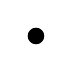
\begin{tikzpicture}[y=0.5cm,x=0.3415cm]
\fill (0,0) circle (3pt);
\end{tikzpicture} \\
$T_1 = 1$
\end{center}
\end{minipage}
\begin{minipage}{1.1in}
\begin{center}
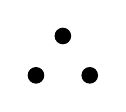
\begin{tikzpicture}[y=0.5cm,x=0.3415cm]
\fill (0,0) circle (3pt);
\fill (1,-1) circle (3pt);
\fill (-1,-1) circle (3pt);
\end{tikzpicture} \\
$T_2 = 3$
\end{center}
\end{minipage}
\begin{minipage}{1.2in}
\begin{center}
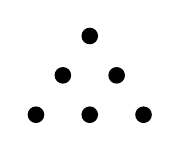
\begin{tikzpicture}[y=0.5cm,x=0.3415cm]
\fill (0,0) circle (3pt);
\fill (1,-1) circle (3pt);
\fill (-1,-1) circle (3pt);
\fill (-2,-2) circle (3pt);
\fill (0,-2) circle (3pt);
\fill (2,-2) circle (3pt);
\end{tikzpicture} \\
$T_3 = 6$
\end{center}
\end{minipage}
\begin{minipage}{1.3in}
\begin{center}
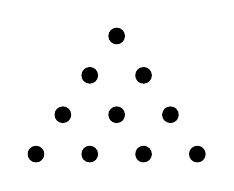
\begin{tikzpicture}[y=0.5cm,x=0.3415cm]
\fill (0,0) circle (3pt);
\fill (1,-1) circle (3pt);
\fill (-1,-1) circle (3pt);
\fill (-2,-2) circle (3pt);
\fill (0,-2) circle (3pt);
\fill (2,-2) circle (3pt);
\fill (-3,-3) circle (3pt);
\fill (-1,-3) circle (3pt);
\fill (1,-3) circle (3pt);
\fill (3,-3) circle (3pt);
\end{tikzpicture} \\
$T_4 = 10$
\end{center}
\end{minipage}
\begin{minipage}{1.5in}
\begin{center}
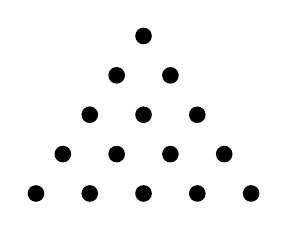
\begin{tikzpicture}[y=0.5cm,x=0.3415cm]
\fill (0,0) circle (3pt);
\fill (1,-1) circle (3pt);
\fill (-1,-1) circle (3pt);
\fill (-2,-2) circle (3pt);
\fill (0,-2) circle (3pt);
\fill (2,-2) circle (3pt);
\fill (-3,-3) circle (3pt);
\fill (-1,-3) circle (3pt);
\fill (1,-3) circle (3pt);
\fill (3,-3) circle (3pt);
\fill (-4,-4) circle (3pt);
\fill (-2,-4) circle (3pt);
\fill (0,-4) circle (3pt);
\fill (2,-4) circle (3pt);
\fill (4,-4) circle (3pt);
\end{tikzpicture} \\
$T_5 = 15$ \\
\end{center}
\end{minipage}
\begin{minipage}{1.7in}
\begin{center}
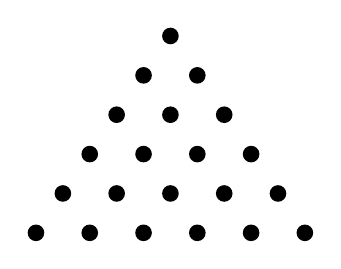
\begin{tikzpicture}[y=0.5cm,x=0.3415cm]
\fill (0,0) circle (3pt);
\fill (1,-1) circle (3pt);
\fill (-1,-1) circle (3pt);
\fill (-2,-2) circle (3pt);
\fill (0,-2) circle (3pt);
\fill (2,-2) circle (3pt);
\fill (-3,-3) circle (3pt);
\fill (-1,-3) circle (3pt);
\fill (1,-3) circle (3pt);
\fill (3,-3) circle (3pt);
\fill (-4,-4) circle (3pt);
\fill (-2,-4) circle (3pt);
\fill (0,-4) circle (3pt);
\fill (2,-4) circle (3pt);
\fill (4,-4) circle (3pt);
\fill (-5,-5) circle (3pt);
\fill (-3,-5) circle (3pt);
\fill (-1,-5) circle (3pt);
\fill (1,-5) circle (3pt);
\fill (3,-5) circle (3pt);
\fill (5,-5) circle (3pt);
\end{tikzpicture} \\
$T_6 = 21$ \\
\end{center}
\end{minipage}
\vspace{12pt}

\caption{The first six triangular numbers}
\end{figure*}
\end{fullwidth}

There are a couple of ways of making this discussion more precise.
Given an equilateral triangle with $n$ dots to a side, how many more
dots do you need to build the equilateral triangle with $n+1$ dots to
a side?  All you need to do to transform the smaller triangle to the
larger triangle is an additional row of $n+1$ dots placed along any
side.  Therefore,
\[
T_{n+1} = T_n + (n+1).
\]
Since $T_1 = 1$, this recursive definition suffices to determine the
whole sequence.

But there are other ways of computing $T_n$.  Indeed, you may recall
the explicit formula
$$
T_n = \frac{n \cdot (n+1)}{2}
$$
from Calculus One.

\subsection{Fibonacci numbers}

\marginnote{The Fibonacci numbers are interesting enough that a
  journal, \href{http://www.fq.math.ca/}{The Fibonacci Quarterly} is
  published four times yearly entirely on topics related to the
  Fibonacci numbers.}

The \defnword{Fibonacci numbers} are defined recursively, starting with
$$
F_0 = 0 \mbox{ and } F_1 = 1
$$
and the rule that $F_{n} = F_{n-1} + F_{n-2}$.  We can restate this
formula in words, instead of symbols; stated in words, each term is
the sum of the previous two terms.  So the sequence of Fibonacci
numbers begins 
$$
0, \quad 1, \quad 1, \quad 2, \quad 3, \quad 5, \quad 8, \quad 13, \quad 21, \quad 34, \quad\ldots
$$
and continues.

This is certainly not the last time we will see the Fibonacci numbers.

\subsection{Collatz sequence}

Here is a fun sequence with which to amuse your friends---or distract
your enemies.  Let's start our sequence with $a_1 = 6$.  Subsequent
terms are defined using the rule
$$
a_n = \begin{cases} a_{n-1} / 2 & \mbox{ if $a_{n-1}$ is even, and } \\
3 \, a_{n-1} + 1 & \mbox{ if $a_{n-1}$ is odd.}
\end{cases}
$$
Let's compute $a_2$.  Since $a_1$ is even, we follow the instructions
in the first line, to find that $a_2 = a_1/2 = 3$. To compute $a_3$,
note that $a_2$ is odd so we follow the instruction in the second
line, and $a_3 = 3 \, a_2 + 1 = 3 \cdot 3 + 1 = 10$.  Since $a_3$ is
even, the first line applies, and $a_4 = a_3 / 2 = 10 / 2 = 5$.  But
$a_4$ is odd, so the second line applies, and we find $a_5 = 3 \cdot 5
+ 1 = 16$.  And $a_5$ is even, so $a_6 = 16 / 2 = 8$.  And $a_6$ is
even, so $a_7 = 8/4 = 4$.  And $a_7$ is even, so $a_8 = 4 / 2 = 2$,
and then $a_9 = 2/2 = 1$.  Oh, but $a_9$ is odd, so $a_{10} = 3 \cdot
1 + 1 = 4$.  And it repeats.  Let's write down the start of this sequence:
$$
6,\quad %1 
3,\quad %2
10,\quad  %3
5,\quad  %4
16,\quad  %5
8,\quad  %6
4,\quad  %7
2,\quad  %8
1,\quad  %9
4,\quad %10
2,\quad %11
1,\quad %12
\overbrace{4,\quad %10
2,\quad %11
1,}^{\mbox{repeats}}\quad %12
4,\quad %10
\ldots
$$
What if we had started with a number other than six?  What if we set
$a_1 = 25$ but then we used the same rule?  In that case, since $a_1$
is odd, we compute $a_2$ by finding $3 \, a_1 + 1 = 3 \cdot 25 + 1 =
76$.  Since $76$ is even, the next term is half that, meaning $a_3 =
38$.  If we keep this up, we find that our sequence begins
\begin{align*}
&25,\quad 76,\quad 38,\quad 19,\quad 58,\quad 29,\quad 88,\quad 44,\quad 22,\quad 11,\quad 34,\quad 17,\quad 52,\quad 26, \\
&13,\quad 40,\quad 20,\quad 10,\quad 5,\quad 16,\quad 8,\quad 4,\quad 2, \quad 1, \quad \ldots
\end{align*}
and then it repeats ``4, 2, 1, 4, 2, 1, \ldots'' just like before.

\marginnote{If you think you have an argument that answers the Collatz conjecture, I challenge you to try your hand at the $5x+1$ conjecture, that is, use the rule
$
a_n = \displaystyle\begin{cases} a_{n-1} / 2 & \mbox{ if $a_{n-1}$ is even, and } \\
5 \, a_{n-1} + 1 & \mbox{ if $a_{n-1}$ is odd.}
\end{cases}
$}

Does this always happen?  Is it true that no matter which positive
integer you start with, if you apply the half-if-even, $3x+1$-if-odd
rule, you end up getting stuck in the ``4, 2, 1, \ldots'' loop?  That
this is true is the \defnword{Collatz conjecture}; it has been
verified for all starting values below $5 \times 2^{60}$.  Nobody has
found a value which doesn't return to one, but for all anybody knows
there \textit{might} well be a very large initial value which doesn't
return to one; nobody knows either way.  It is an unsolved
problem\sidenote{This is not the last unsolved problems we will
  encounter in this course.  There are many things which humans do not
  understand.} in mathematics.

\section{Where is a sequence headed?  Take a limit!}
\label{section:limits}

We've seen a lot of sequences, and already there are a few things we
might notice.  For instance, the arithmetic progression
$$
1,\quad 8,\quad 15,\quad 22,\quad 29,\quad 36,\quad 43,\quad 50,\quad 57,\quad 64,\quad 71,\quad 78,\quad 85,\quad 92,\quad \ldots
$$
just keeps getting bigger and bigger.  No matter how large a number
you think of, if I add enough $7$'s to $1$, eventually I will surpass
the giant number you thought of.  On the other hand, the terms in a geometric progression where each term is half the previous term, namely
$$
\frac{1}{2},\quad \frac{1}{4},\quad \frac{1}{8},\quad \frac{1}{16},\quad \frac{1}{32},\quad \frac{1}{64},\quad \frac{1}{128},\quad \frac{1}{256},\quad \frac{1}{512},\quad \frac{1}{1024},\quad \ldots ,
$$
are getting closer and closer to zero.  No matter how close you stand
near but not at zero, eventually this geometric sequence gets even closer than you
are to zero.

These two sequences have very different stories.  One shoots off to
infinity; the other zooms in towards zero.  Mathematics is not just
about numbers; mathematics provides tools for talking about the
qualitative features of the numbers we deal with.  What about the two
sequences we just considered?  They are qualitatively very different.  The first ``goes to''
infinity; the second ``goes to'' zero.

\marginnote{If you were with us in Calculus One, you are perhaps
  already guessing that by ``goes to,'' I actually mean ``has
  limit.''}

In short, given a sequence, it is helpful to be able to say something
qualitative about it; we may want to address the question such as
``what happens after a while?'' Formally, when faced with a sequence,
we are interested in the limit
$$\lim_{i\to \infty} f(i) = \lim_{i\to\infty} a_i.$$
In Calculus One, we studied a similar question about
$$\lim_{x\to\infty} f(x)$$
when $x$ is a variable taking on real values; now, in Calculus Two, we
simply want to restrict the ``input'' values to be integers. No
significant difference is required in the definition of limit, except
that we specify, perhaps implicitly, that the variable is an integer.

\begin{definition} \relax\index{limit of a sequence}
Suppose that $\left(a_n\right)$ is a sequence.
To say that $\ds \lim_{n\to \infty}a_n=L$ is to say that \\
\null\quad for every $\epsilon>0$, \\
\null\quad\quad there is an $N > 0$, \\
\null\quad so that whenever $n>N$, \\
\null\quad\quad we have $|a_n-L|<\epsilon$. \\
If $\ds \lim_{n\to\infty}a_n=L$ we say that the sequence
\defnword{converges}\index{convergent
  sequence}\index{sequence!convergent}.  If there is no finite value $L$ so
that $\ds \lim_{n\to\infty}a_n = L$, then we say that the limit
\defnword{does not exist}, or equivalently that the sequence
\defnword{diverges}\index{divergent sequence}\index{sequence!divergent}.
\end{definition} 

\marginnote{The definition of limit is being written as if it were
  poetry, what with line breaks and all.  Like the best of poems, it deserves to be memorized, performed, internalized.  Humanity struggled for millenia to find the wisdom contained therein.}

\begin{warning}
  In the case that $\lim_{n \to \infty} a_n = \infty$, we say that
  $(a_n)$ diverges, or perhaps more precisely, we say $(a_n)$ diverges to
  infinity.  The only time we say that a sequence converges is when
  the limit exists and is equal to a \textit{finite} value.
\end{warning}

One way to compute the limit of a sequence is to compute the limit of
a function.
\begin{theorem}
  Let $f(x)$ be a real-valued function.  If $a_n = f(n)$ defines a
  sequence $(a_n)$ and if $\ds \lim_{x\to\infty}f(x)=L$ in the sense of Calculus
  One, then $\ds \lim_{n\to\infty} a_n=L$ as well.
\end{theorem}

\begin{example}
Since $\ds \lim_{x\to\infty}(1/x)=0$, it is
clear that also $\ds \lim_{n\to\infty}(1/n)=0$; in other words, the sequence of numbers
$${1\over1},\quad {1\over2},\quad {1\over3},\quad {1\over4},\quad {1\over5},\quad {1\over6},\quad \ldots$$
get closer and closer to 0, or more precisely, as close as you want to get to zero, after a while, all the terms in the sequence are that close.
\end{example}


But it is important to note that the converse\sidenote{\label{sidenote:raining-converse}The
  \defnword{converse} of a statement is what you get when you swap the
  assumption and the conclusion; the converse of ``if it is raining,
  then it is cloudy'' is the statement ``if it is cloudy, then it is
  raining.''  Which of those statements is true?} of this theorem is
not true.  To show the converse is not true, it is enough to provide a
single example where it fails.  Here's the counterexample\sidenote{An
  instance of (a potential) general rule being broken is called a
  \defnword{counterexample}.  This is a popular term among mathematicians and philosophers.}.

\begin{example}
  Consider the sequence $(a_n)$ given by the rule $a_n = f(n)=\sin(n\pi)$.  This is the sequence
$$
  \sin(0\pi),\quad \sin(1\pi),\quad\sin(2\pi),\quad\sin(3\pi),\quad\ldots,
$$
which is just the sequence $0, 0, 0, 0, \ldots$ since $\sin(n\pi)=0$
whenever $n$ is an integer.  Since the sequence is just the constant sequence, we have
$$
\lim_{n\to\infty} f(n)= \lim_{n\to\infty} 0 = 0. 
$$But $\ds \lim_{x\to\infty}f(x)$, when $x$ is real, does not exist: as $x$ gets
bigger and bigger, the values $\sin(x\pi)$ do not get closer and
closer to a single value, but instead oscillate between $-1$ and $1$.
\end{example} 

Here's some general advice. If you want to know $\ds \lim_{n\to\infty}
a_n$, you might first think of a function $f(x)$ where $a_n = f(n)$,
and then attempt to compute $\ds \lim_{x\to\infty}f(x)$.  If the limit
of the function exists, then it is equal to the limit of the sequence.
But, if for some reason $\ds \lim_{x\to\infty}f(x)$ does not exist, it
may nevertheless still be the case that $\ds \lim_{n\to\infty}f(n)$
exists---you'll just have to figure out another way to compute it.


\begin{marginfigure}[0in]
\begin{tikzpicture}
	\begin{axis}[
            domain=0:20,
            ymax=2.25,
            ymin=-1.5,
            xmin=0,
            xmax=20.25,
            axis lines =middle, xlabel={$x$ and $n$}, ylabel=$y$,
            every axis y label/.style={at=(current axis.above origin),anchor=south},
            every axis x label/.style={at=(current axis.right of origin),anchor=west}
          ]
%scale = 10 ; print(join([str((n(x/scale,digits=5),n(cos(pi*(x/scale)) + (4/5)^(x/scale),digits=5))) for x in range(1,20*scale)],' '))
          \addplot [penColor, smooth] plot coordinates { (0.50000, 0.89443) (0.60000, 0.56567) (0.70000, 0.26760) (0.80000, 0.027494) (0.90000, -0.13300) (1.0000, -0.20000) (1.1000, -0.16871) (1.2000, -0.043935) (1.3000, 0.16041) (1.4000, 0.42267) (1.5000, 0.71554) (1.6000, 1.0088) (1.7000, 1.2721) (1.8000, 1.4782) (1.9000, 1.6055) (2.0000, 1.6400) (2.1000, 1.5769) (2.2000, 1.4211) (2.3000, 1.1863) (2.4000, 0.89437) (2.5000, 0.57243) (2.6000, 0.25078) (2.7000, -0.040337) (2.8000, -0.27365) (2.9000, -0.42750) (3.0000, -0.48800) (3.1000, -0.45035) (3.2000, -0.31936) (3.3000, -0.10893) (3.4000, 0.15926) (3.5000, 0.45795) (3.6000, 0.75686) (3.7000, 1.0258) (3.8000, 1.2373) (3.9000, 1.3699) (4.0000, 1.4096) (4.1000, 1.3516) (4.2000, 1.2007) (4.3000, 0.97085) (4.4000, 0.68364) (4.5000, 0.36636) (4.6000, 0.049256) (4.7000, -0.23742) (4.8000, -0.46638) (4.9000, -0.61598) (5.0000, -0.67232) (5.1000, -0.63061) (5.2000, -0.49564) (5.3000, -0.28131) (5.4000, -0.0093174) (5.5000, 0.29309) (5.6000, 0.59564) (5.7000, 0.86808) (5.8000, 1.0831) (5.9000, 1.2191) (6.0000, 1.2621) (6.1000, 1.2074) (6.2000, 1.0597) (6.3000, 0.83294) (6.4000, 0.54878) (6.5000, 0.23447) (6.6000, -0.079722) (6.7000, -0.36355) (6.8000, -0.58973) (6.9000, -0.73661) (7.0000, -0.79029) (7.1000, -0.74597) (7.2000, -0.60845) (7.3000, -0.39163) (7.4000, -0.11721) (7.5000, 0.18757) (7.6000, 0.49245) (7.7000, 0.76718) (7.8000, 0.98445) (7.9000, 1.1226) (8.0000, 1.1678) (8.1000, 1.1151) (8.2000, 0.96947) (8.3000, 0.74469) (8.4000, 0.46246) (8.5000, 0.15006) (8.6000, -0.16227) (8.7000, -0.44427) (8.8000, -0.66867) (8.9000, -0.81381) (9.0000, -0.86578) (9.1000, -0.81979) (9.2000, -0.68066) (9.3000, -0.46224) (9.4000, -0.18626) (9.5000, 0.12005) (9.6000, 0.42642) (9.7000, 0.70259) (9.8000, 0.92129) (9.9000, 1.0608) (10.000, 1.1074) (10.100, 1.0560) (10.200, 0.91171) (10.300, 0.68821) (10.400, 0.40722) (10.500, 0.096038) (10.600, -0.21510) (10.700, -0.49595) (10.800, -0.71920) (10.900, -0.86321) (11.000, -0.91410) (11.100, -0.86704) (11.200, -0.72687) (11.300, -0.50745) (11.400, -0.23045) (11.500, 0.076831) (11.600, 0.38415) (11.700, 0.66128) (11.800, 0.88087) (11.900, 1.0213) (12.000, 1.0687) (12.100, 1.0182) (12.200, 0.87474) (12.300, 0.65205) (12.400, 0.37187) (12.500, 0.061465) (12.600, -0.24891) (12.700, -0.52903) (12.800, -0.75153) (12.900, -0.89484) (13.000, -0.94502) (13.100, -0.89728) (13.200, -0.75644) (13.300, -0.53635) (13.400, -0.25874) (13.500, 0.049172) (13.600, 0.35710) (13.700, 0.63484) (13.800, 0.85501) (13.900, 0.99603) (14.000, 1.0440) (14.100, 0.99405) (14.200, 0.85108) (14.300, 0.62889) (14.400, 0.34924) (14.500, 0.039337) (14.600, -0.27055) (14.700, -0.55015) (14.800, -0.77223) (14.900, -0.91508) (15.000, -0.96482) (15.100, -0.91663) (15.200, -0.77537) (15.300, -0.55485) (15.400, -0.27684) (15.500, 0.031470) (15.600, 0.33979) (15.700, 0.61788) (15.800, 0.83845) (15.900, 0.97983) (16.000, 1.0281) (16.100, 0.97856) (16.200, 0.83594) (16.300, 0.61412) (16.400, 0.33476) (16.500, 0.025176) (16.600, -0.28440) (16.700, -0.56376) (16.800, -0.78547) (16.900, -0.92802) (17.000, -0.97748) (17.100, -0.92903) (17.200, -0.78748) (17.300, -0.56673) (17.400, -0.28842) (17.500, 0.020141) (17.600, 0.32871) (17.700, 0.60711) (17.800, 0.82785) (17.900, 0.96947) (18.000, 1.0180) (18.100, 0.96867) (18.200, 0.82625) (18.300, 0.60463) (18.400, 0.32549) (18.500, 0.016113) (18.600, -0.29326) (18.700, -0.57244) (18.800, -0.79395) (18.900, -0.93632) (19.000, -0.98559) (19.100, -0.93695) (19.200, -0.79523) (19.300, -0.57430) (19.400, -0.29584) (19.500, 0.012890) (19.600, 0.32162) (19.700, 0.60019) (19.800, 0.82107) (19.900, 0.96285)};
          \node at (axis cs:2.2000, 1.4211) [anchor=south west] {\color{penColor}$f(x)$};  
          \node at (axis cs:10, 1.15) [anchor=south] {\color{penColor2}$a_n$};
% print(join([str((x,n(cos(pi*x) + (4/5)^x,digits=5))) for x in range(1,20)],' ')) 
          \addplot[color=penColor2,fill=penColor2,only marks,mark=*] coordinates{(1, -0.20000) (2, 1.6400) (3, -0.48800) (4, 1.4096) (5, -0.67232) (6, 1.2621) (7, -0.79029) (8, 1.1678) (9, -0.86578) (10, 1.1074) (11, -0.91410) (12, 1.0687) (13, -0.94502) (14, 1.0440) (15, -0.96482) (16, 1.0281) (17, -0.97748) (18, 1.0180) (19, -0.98559) (20, 1.0115)};

        \end{axis}
\end{tikzpicture}
\caption{Plots of $f(x) = \cos (\pi \, x) + (4/5)^x$ and the sequence $a_n = (-1)^n + (4/5)^n$.}
\label{fig:graphs-of-sequences}
\end{marginfigure}

\section{Graphs}
\label{section:graphs}

It is occasionally useful to think of the graph of a sequence. Since
the function is defined only for integer values, the graph is just a
sequence of dots. In Figure~\xrefn{fig:graphs-of-sequences} we see the
graph of a sequence and the graph of a corresponding real-valued
function.

There are lots of real-valued functions which ``fill in'' the missing
values of a sequence.

\begin{example}
  Here's a particularly tricky example of ``filling in'' the missing values of a sequence.  Consider the sequence
  $$
  1,\quad 2,\quad 6,\quad 24,\quad 120,\quad 720,\quad 5040,\quad 40320,\quad 362880,\quad\ldots,
  $$
  where the $n^{\nth}$ term is the product of the first $n$ integers.
  In other words $a_n = n!$, where the exclamation mark denotes the
  \defnword{factorial} function.  Explicitly describe a function $f$
  of a real variable $x$, so that $a_n = f(n)$ for natural numbers
  $n$.
\end{example}

\begin{marginfigure}[0in]
\begin{tikzpicture}
	\begin{axis}[
            domain=0:4.2,
            ymax=25,
            ymin=-0.1,
            xmin=0,
            xmax=4.2,
            axis lines =middle, xlabel={$x$ and $n$}, ylabel=$y$,
            every axis y label/.style={at=(current axis.above origin),anchor=south},
            every axis x label/.style={at=(current axis.right of origin),anchor=west}
          ]
          \node at (axis cs:2.5, 3) [anchor=south] {\color{penColor}$f(x)$};  
          \addplot [very thick, penColor, domain=(0:1)] {1};
          \addplot [very thick, penColor, domain=(1:2)] {1};
          \addplot [very thick, penColor, domain=(2:3)] {2};
          \addplot [very thick, penColor, domain=(3:4)] {6};
          \addplot [very thick, penColor, domain=(4:5)] {24};
          \addplot[color=penColor,fill=penColor,only marks,mark=*] coordinates{(1, 1) (2, 2) (3, 6) (4, 24)};
          \addplot[color=penColor,fill=background,only marks,mark=*] coordinates{(2, 1) (3, 2) (4, 6) (5, 24)};
% print(join([str((x,factorial(x))) for x in range(1,20)],' ')) 
          \addplot[color=penColor2,fill=penColor2,only marks,mark=*] coordinates{(1, 1) (2, 2) (3, 6) (4, 24)};
          \node at (axis cs:3, 7) [anchor=south] {\color{penColor2}$a_n$};
        \end{axis}
\end{tikzpicture}
\caption{A plot of $f(x) = \floor{x}!$ and $a_n = n!$.  Recall that, by convention, $0! = 1$.}
\label{fig:floor-graph}
\end{marginfigure}


\begin{solution}
  There are lots of solutions.  Here is a solution:
$$
f(x) = \floor{x}!.
$$
In that definition, $\floor{x}$ denotes the ``greatest integer less
  than or equal to $x$'' and is called the \defnword{floor function}.  This is shown in Figure~\xrefn{fig:floor-graph}.

  On the other hand, there are much trickier things that you could try
  to do.  If you define the \defnword{Gamma function}
  $$
  \Gamma(z) = \int_0^\infty t^{z-1} e^{-t} \, dt.
  $$
  then it is perhaps very surprising to find out that $g(x) =
  \Gamma(x+1)$ is a function so that $g(n) = n!$ for natural numbers
  $n$.  A graph is shown in Figure~\xrefn{fig:gamma-function}.
  Unlike $f$, which fails to be continuous, the function $g$ is continuous.
\end{solution}

\marginnote{It is hard to define the ``greatest integer'' function,
  because they are all pretty great.}

\begin{marginfigure}[0in]
\begin{tikzpicture}
	\begin{axis}[
            domain=0:4.2,
            ymax=25,
            ymin=-0.1,
            xmin=0,
            xmax=4.2,
            axis lines =middle, xlabel={$x$ and $n$}, ylabel=$y$,
            every axis y label/.style={at=(current axis.above origin),anchor=south},
            every axis x label/.style={at=(current axis.right of origin),anchor=west}
          ]
%scale = 30 ; print(join([str((n(x/scale,digi>s=5),n(gamma(x/scale + 1),digits=5))) for x in range(0,4.2*scale)],' '))
\addplot [penColor, smooth] plot coordinates { 
(0.00000, 1.0000) (0.033333, 0.98183) (0.066667, 0.96566) (0.10000, 0.95135) (0.13333, 0.93874) (0.16667, 0.92772) (0.20000, 0.91817) (0.23333, 0.91000) (0.26667, 0.90312) (0.30000, 0.89747) (0.33333, 0.89298) (0.36667, 0.88959) (0.40000, 0.88726) (0.43333, 0.88595) (0.46667, 0.88561) (0.50000, 0.88623) (0.53333, 0.88776) (0.56667, 0.89020) (0.60000, 0.89352) (0.63333, 0.89770) (0.66667, 0.90275) (0.70000, 0.90864) (0.73333, 0.91538) (0.76667, 0.92296) (0.80000, 0.93138) (0.83333, 0.94066) (0.86667, 0.95078) (0.90000, 0.96177) (0.93333, 0.97362) (0.96667, 0.98636) (1.0000, 1.0000) (1.0333, 1.0146) (1.0667, 1.0300) (1.1000, 1.0465) (1.1333, 1.0639) (1.1667, 1.0823) (1.2000, 1.1018) (1.2333, 1.1223) (1.2667, 1.1440) (1.3000, 1.1667) (1.3333, 1.1906) (1.3667, 1.2158) (1.4000, 1.2422) (1.4333, 1.2699) (1.4667, 1.2989) (1.5000, 1.3293) (1.5333, 1.3612) (1.5667, 1.3946) (1.6000, 1.4296) (1.6333, 1.4662) (1.6667, 1.5046) (1.7000, 1.5447) (1.7333, 1.5867) (1.7667, 1.6306) (1.8000, 1.6765) (1.8333, 1.7245) (1.8667, 1.7748) (1.9000, 1.8274) (1.9333, 1.8823) (1.9667, 1.9398) (2.0000, 2.0000) (2.0333, 2.0629) (2.0667, 2.1287) (2.1000, 2.1976) (2.1333, 2.2697) (2.1667, 2.3451) (2.2000, 2.4240) (2.2333, 2.5065) (2.2667, 2.5930) (2.3000, 2.6834) (2.3333, 2.7782) (2.3667, 2.8773) (2.4000, 2.9812) (2.4333, 3.0900) (2.4667, 3.2040) (2.5000, 3.3233) (2.5333, 3.4485) (2.5667, 3.5796) (2.6000, 3.7170) (2.6333, 3.8611) (2.6667, 4.0122) (2.7000, 4.1707) (2.7333, 4.3369) (2.7667, 4.5112) (2.8000, 4.6942) (2.8333, 4.8862) (2.8667, 5.0877) (2.9000, 5.2993) (2.9333, 5.5215) (2.9667, 5.7549) (3.0000, 6.0000) (3.0333, 6.2575) (3.0667, 6.5282) (3.1000, 6.8126) (3.1333, 7.1116) (3.1667, 7.4260) (3.2000, 7.7567) (3.2333, 8.1044) (3.2667, 8.4704) (3.3000, 8.8554) (3.3333, 9.2606) (3.3667, 9.6871) (3.4000, 10.136) (3.4333, 10.609) (3.4667, 11.107) (3.5000, 11.632) (3.5333, 12.185) (3.5667, 12.767) (3.6000, 13.381) (3.6333, 14.029) (3.6667, 14.711) (3.7000, 15.431) (3.7333, 16.191) (3.7667, 16.992) (3.8000, 17.838) (3.8333, 18.730) (3.8667, 19.673) (3.9000, 20.667) (3.9333, 21.718) (3.9667, 22.828) (4.0000, 24.000) (4.0333, 25.239) (4.0667, 26.548) (4.1000, 27.932) (4.1333, 29.395) (4.1667, 30.942)};
          \node at (axis cs:2.5, 3.3233) [anchor=south east] {\color{penColor}$f(x)$};  
% print(join([str((x,factorial(x))) for x in range(1,20)],' ')) 
          \addplot[color=penColor2,fill=penColor2,only marks,mark=*] coordinates{(1, 1) (2, 2) (3, 6) (4, 24)};
          \node at (axis cs:3, 7) [anchor=north west] {\color{penColor2}$a_n$};
        \end{axis}
\end{tikzpicture}
\caption{Plots of $f(x) = \int_0^\infty t^{z} e^{-t} \, dt.$ and $a_n = n!$.}
\label{fig:gamma-function}
\end{marginfigure}

\section{New sequences from old}
\label{section:new-sequences-from-old}

Given a sequence, one way to build a new sequence is to start with the
old sequence, but then throw away a whole bunch of terms.  For
instance, if we started with the sequence of perfect squares
$$
1,\quad 4,\quad 9,\quad 16,\quad 25,\quad 36,\quad 49,\quad 64,\quad 81,\quad\ldots
$$
we could throw away all the odd-indexed terms, and be left with
$$
4,\quad 16,\quad 36,\quad 64,\quad 100,\quad 144,\quad 196,\quad 256,\quad 324,\quad 400,\quad 484,\quad\ldots
$$
We say that this latter sequence is a
\defnword{subsequence}\index{sequence!subsequence}\index{subsequence}
of the original sequence.  Here is a precise definition.

\begin{definition}
  Suppose $(a_n)$ is a sequence with initial index $N$, and suppose we have a sequence of integers $(n_i)$ so that
  $$
  N \leq n_1 < n_2 < n_3 < n_4 < n_5 < \cdots 
  $$
  Then the sequence $(b_i)$ given by $b_i = a_{n_i}$ is said to be a \defnword{subsequence}\index{sequence!subsequence}\index{subsequence}
  of the sequence $a_n$.
\end{definition}

Limits are telling the story of ``what happens'' to a sequence.  If
the terms of a sequence can be made as close as desired to a limiting
value $L$, then the subsequence must share that same fate.

\begin{theorem}
  \label{theorem:subsequence-same-limit}
  If $(b_i)$ is a subsequence of the convergent sequence $(a_n)$, then
  $\ds\lim_{i \to \infty} b_i = \ds\lim_{n \to \infty} a_n$.
\end{theorem}

Of course, just because a subsequence converges does not mean that the
larger sequence converges, too.  We'll see this again in more detail
when we get to Example~\xrefn{example:alternating-ones}, but we'll
discuss it briefly now.

\begin{example}
Find a convergent subsequence of the sequence $(a_n)$ given by the rule $a_n = (-1)^n$.
\end{example}

\begin{solution}
Note that the sequence $(a_n)$ does not converge.  But by considering the sequence of indexes $n_i = 2 \cdot i$, we can build a subsequence
$$
b_i = a_{n_i} = a_{2i} = (-1)^{2i} = 1,
$$
which is a constant sequence, so it converges to 1.
\end{solution}

There are other subsequences of $a_n = (-1)^n$ which converge but do
\textit{not} converge to one.  For instance, the subsequence of odd
indexed terms is the constant sequence $c_n = -1$, which converges to
$-1$.  For that matter, the fact that there are convergent
subsequences with distinct limits perhaps explains why the original
sequence $(a_n)$ does not converge.  Let's formalize this.

\begin{corollary}
  \label{corollary:different-subsequences-then-diverge}

  Suppose $(b_i)$ and $(c_i)$ are convergent subsequences of the sequence $(a_n)$, but
  $$
  \ds\lim_{i \to \infty} b_i \neq \ds\lim_{n \to \infty} c_i.
  $$
  Then the sequence $(a_n)$ does not converge.
\end{corollary}

\begin{proof}
  Suppose, on the contrary, the sequence $(a_n)$ did converge.  Then by
  Theorem~\xrefn{theorem:subsequence-same-limit}, the subsequence
  $(b_i)$ would converge, too, and
  $$
  \ds\lim_{i \to \infty} b_i = \ds\lim_{n \to \infty} a_n.
  $$
  Again by Theorem~\xrefn{theorem:subsequence-same-limit}, the subsequence
  $(c_i)$ would converge, too, and
  $$
  \ds\lim_{i \to \infty} c_i = \ds\lim_{n \to \infty} a_n.
  $$
  But then $\ds\lim_{i \to \infty} b_i = \ds\lim_{i \to \infty} c_i$,
  which is exactly what we are supposing doesn't happen!  To avoid
  this contradiction, it must be that our original assumption that
  $(a_n)$ converged was incorrect; in short, the sequence $(a_n)$ does
  not converge.
\end{proof}

\section{Helpful theorems about limits}
\label{section:theorems-about-limits}

Not surprisingly, the properties of limits of real functions translate
into properties of sequences quite easily. 

%\vbox{
\begin{theorem} \relax\label{thm:properties-of-sequences}
Suppose that $\ds\lim_{n\to\infty}a_n=L$ and 
$\ds\lim_{n\to\infty}b_n=M$ and
$k$ is some constant. Then
\begin{align*}
&\lim_{n\to\infty} ka_n = k\lim_{n\to\infty}a_n=kL, \\
&\lim_{n\to\infty} (a_n+b_n) = \lim_{n\to\infty}a_n+\lim_{n\to\infty}b_n=L+M, \\
&\lim_{n\to\infty} (a_n-b_n) = \lim_{n\to\infty}a_n-\lim_{n\to\infty}b_n=L-M, \\
&\lim_{n\to\infty} (a_nb_n) = \lim_{n\to\infty}a_n\cdot\lim_{n\to\infty}b_n=LM, \mbox{ and}\\
&\lim_{n\to\infty} {a_n\over b_n} = {\lim_{n\to\infty}a_n\over
  \lim_{n\to\infty}b_n}={L\over M},\hbox{ provided $M \neq 0$.} \\
\end{align*}
\end{theorem}
%}

\subsection{Squeeze Theorem}

Likewise, there is an analogue of the squeeze theorem for functions.

\begin{theorem}\relax\label{thm:squeeze theorem for sequences}
Suppose there is some $N$ so that for all $n > N$, it is the case that $\ds a_n \le b_n \le c_n$. If $$\ds\lim_{n\to\infty}a_n=\ds\lim_{n\to\infty}c_n=L$$, 
then $\ds\lim_{n\to\infty}b_n=L$.
\end{theorem}

And a final useful fact:

\begin{theorem} \relax\label{thm:absolute value sequence}
$\ds\lim_{n\to\infty}|a_n|=0$ if and only if
$\ds\lim_{n\to\infty}a_n=0$.
\end{theorem}
\marginnote{Sometimes people write ``iff'' as shorthand for ``if and only if.''}

This says simply that the size of $\ds a_n$ gets close to zero if and
only if $\ds a_n$ gets close to zero.

\subsection{Examples}

Armed with these helpful theorems, we are now in a position to work a
number of examples.

\begin{example}
Determine whether the sequence $(a_n)$ given by the rule $a_n = \frac{n}{n+1}$ converges or
diverges. If it converges, compute the limit.
\end{example}

\begin{solution}
Consider the real-valued function
$$
f(x) = \frac{x}{x+1}.
$$
Since $a_n = f(n)$, it will be enough to find $\ds\lim_{x \to \infty} f(x)$ in order to find $\ds\lim_{n \to \infty} a_n$.
We compute, as in Calculus One, that
\begin{align*}
\lim_{x\to\infty}{x\over x+1}
&= \lim_{x\to\infty} \frac{(x+1) - 1}{x+1} \\
&= \lim_{x\to\infty} \left( \frac{x+1}{x+1} - \frac{1}{x+1} \right) \\
&= \lim_{x\to\infty} \left( 1 - \frac{1}{x+1} \right) \\
&= \lim_{x\to\infty} 1 - \lim_{x \to \infty} \frac{1}{x+1} \\
&= 1 - \lim_{x \to \infty} \frac{1}{x+1} = 1 - 0 = 1. \\
\end{align*}
We therefore conclude that $\ds\lim_{n \to \infty} a_n = 1$.
\end{solution}
\marginnote{And this is reasonable: by choosing $n$ to be a large enough integer, I can make $\ds\frac{n}{n+1}$ as close to $1$ as I would like.  Just imagine how close $\frac{10000000000}{10000000001}$ is to one.}

\begin{example}
\label{example:log-n-over-n}
Determine whether the sequence $(a_n)$ given by $\ds a_n = \frac{\log n}{n}$ converges or
diverges.  If it converges, compute the limit.
\end{example}

\begin{solution}
By l'H\^opital's rule, we compute
$$\lim_{x\to\infty}{\log x\over x}=\lim_{x\to\infty}{1/x\over 1}=
0.$$
Therefore, $$\lim_{n \to \infty}  \frac{\log n}{n} = 0.$$
\end{solution}

\marginnote{I'm not too fond of l'H\^opital's rule, so I would have
  been happier if I had given a solution that didn't involve it; you
  could avoid mentioning l'H\^opital's rule in
  Example~\xrefn{example:log-n-over-n} if you used, say, the squeeze
  theorem and the fact that $\log n \leq \sqrt{n}$.}

\begin{example}
\label{example:alternating-ones}
Determine whether the sequence $(a_n)$ given by the rule $a_n = (-1)^n$ converges or
diverges. If it converges, compute the limit.
\end{example}

\begin{solution}
  Your first inclination might be to consider the ``function'' $f(x) =
  (-1)^x$, but you'll run into trouble when trying to tell me the
  value of $f(1/2)$.

  How does the sequence $a_n = (-1)^n$ begin?  It starts
  $$
-1,\quad
1,\quad
-1,\quad
1,\quad
-1,\quad
1,\quad
-1,\quad
1,\quad
-1,\quad
1,\quad\ldots,
  $$
  so the sequence isn't getting close to any number in particular.

  Intuitively, the above argument is probably pretty convincing.  But
  if you want an airtight argument, you can reason like this:
  suppose---though we'll soon see that this is a ridiculous
  assumption---that the sequence $a_n = (-1)^n$ did converge to $L$.
  Then any subsequence would also converge to $L$, by
  Theorem~\xrefn{theorem:subsequence-same-limit} which stated that the
  limit of a subsequence is the same as the limit of the original
  sequence.  If I throw away every other term of the sequence $(a_n)$,
  I am left with the constant sequence
$$
-1,\quad
-1,\quad
-1,\quad
-1,\quad
-1,\quad
-1,\quad
-1,\quad\ldots,
$$
which converges to $-1$, and so $L$ must be $-1$.

On the other hand, if I throw away all the terms with odd indices and
keep only those terms with even indices, I am left with the constant
subsequence
$$
1,\quad
1,\quad
1,\quad
1,\quad
1,\quad
1,\quad
1,\quad\ldots,
$$
so $L$ must be $1$.  Since $L$ can't be both $-1$ and $1$, it couldn't
have been the case that $\ds\lim_{n \to \infty} a_n = L$ for a real
number $L$.  In other words, the limit does not exist.
\end{solution}

\marginnote{I imagine that the ``airtight argument'' in the solution
  to Example~\xrefn{example:alternating-ones} is difficult to
  understand.  Please don't worry if you find the argument confusing
  now---we'll have more opportunities for doing these sorts of
  \href{http://en.wikipedia.org/wiki/Proof_by_contradiction}{proofs by
    contradiction} in the future.}

\begin{example}
Determine whether the sequence $a_n = (-1/2)^n$ converges or
diverges. If it converges, compute the limit.
\end{example}

\marginnote{In this problem, you must be very careful to recognize the
  difference between $(-1/2)^n$ and $-(1/2)^n$.  The former flip-flops
  between being positive and being negative, while the latter is
  always negative.}

\begin{solution}
  Let's use the Squeeze Theorem.  Consider the sequences $b_n =
  -(1/2)^n$ and $c_n = (1/2)^n$.  Then $b_n \leq a_n \leq c_n$.  And
  $\ds\lim_{n \to \infty} c_n = 0$ because $\lim_{x \to \infty}
  (1/2)^x = 0$.  Since $b_n = - c_n$, we have $\lim_{n \to \infty} b_n
  = - \lim_{n \to \infty} c_n = -0 = 0$.  Since $b_n$ and $c_n$
  converge to zero, the squeeze theorem tells us that $\ds\lim_{n \to
    \infty} a_n = 0$ as well.

  If you don't want to mention the Squeeze Theorem, you could instead
  apply Theorem~\xrefn{thm:absolute value sequence}.  In that case, we
  would again consider the sequence $c_n = |a_n|$ and observe that
  $\ds\lim_{n \to \infty} c_n = 0$.  But then
  Theorem~\xrefn{thm:absolute value sequence} steps in, and tells us
  that $\ds\lim_{n \to \infty} a_n = 0$ as well.  Of course, a
  convincing argument for why Theorem~\xrefn{thm:absolute value
    sequence} works at all goes via the squeeze theorem, so this
  second method is not so different from the first.
\end{solution}

\begin{example}
Determine whether $a_n = \ds\frac{\sin n}{\sqrt{n}}$ converges or
diverges. If it converges, compute the limit. 
\end{example}

\begin{solution}
Since $-1 \leq \sin n \leq 1$, we have 
$$
\frac{-1}{\sqrt{n}} \leq \frac{\sin n}{\sqrt{n}} \leq \frac{1}{\sqrt{n}},
$$ 
and can therefore apply the Squeeze Theorem.  Since $\ds\lim_{x \to \infty} \frac{1}{\sqrt{x}} = 0$, we get
$$
\lim_{n \to \infty} \frac{-1}{\sqrt{n}} = \lim_{n \to \infty} \frac{1}{\sqrt{n}} = 0,
$$
and so by squeezing, we conclude $\ds\lim_{n \to \infty} a_n = 0$.
\end{solution}

\marginnote{You might be wondering why I love the Squeeze Theorem so
  much; one reason is that the Squeeze Theorem gets you into the idea
  of ``comparing'' one sequence to another, and this ``comparison''
  idea will be big when we get to convergence tests in
  Chapter~\xrefn{chapter:convergence-tests}.}

\begin{example}
A particularly common and useful sequence is the geometric progression $a_n = r^n$
for a fixed real number $r$.  For which values of $r$ does this sequence converge?
\end{example}

\begin{solution}
It very much does depend on $r$.

If $r=1$, then $a_n = (1)^n$ is the constant sequence
$$
1,\quad
1,\quad
1,\quad
1,\quad
1,\quad
1,\quad
1,\quad
1,\quad \ldots,
$$
so the sequence converges to one.  A similarly boring fate befalls the
case $r = 0$, in which case $a_n = (0)^n$ converges to zero.

If $r=-1$, we are reprising the sequence which starred in
Example~\xrefn{example:alternating-ones}; as we saw, that sequence
diverges.

If either $r>1$ or $r<-1$, then the terms $a_n = r^n$ can be made as
large as one likes by choosing $n$ large enough (and even), so the
sequence diverges.

If $0<r<1$, then the sequence converges to 0. 

If $-1<r<0$ then $\ds |r^n|=|r|^n$ and $0<|r|<1$, so the sequence
$\ds \{|r|^n\}_{n=0}^\infty$ converges to 0, so also 
$\ds\{r^n\}_{n=0}^\infty$ converges to 0.
\end{solution}

That last example of a geometric progression is involved enough that
it deserves to be summarized as a theorem.

\begin{theorem}
The sequence $a_n = r^n$ converges when
$-1<r \le 1$, and diverges otherwise.  In symbols,
$$
  \lim_{n\to\infty} r^n=\begin{cases}
  0& if $-1<r<1$, \\
  1& if $r=1$, \mbox{ and} \\
  \mbox{does not exist} & \mbox{if $r \leq -1$ or $r > 1$.}
\end{cases}
$$  
\end{theorem}

\section{Qualitative features of sequences}
\label{section:qualitative-features-of-sequences}

\marginnote{Your first exposure to mathematics might have been about
  \defnword{constructions}; you might have been asked to compute a
  numeric answer or to propose a solution to a problem.  But much of
  mathematics is concerned with showing \defnword{existence}, even if
  the thing that is being shown to exist cannot be exhibited itself.}

Sometimes we will not be able to determine the limit of a sequence,
but we still would like to know whether or not it converges to some
unspoken number.  In many cases, we can determine whether a limit
exists, without needing to---or without even being able to---compute
that limit.

\subsection{Monotonicity}
\label{subsection:monotonicity}

And sometimes we don't even care about limits, but we'd simply like
some terminology with which to describe features we might notice about
sequences.  Here is some of that terminology.

\marginnote{For instance, how much money I have on day $n$ is a
  sequence; I probably hope that sequence is an increasing sequence.}

\begin{definition}
  A sequence is called
  \defnword{increasing}\index{sequence!increasing} (or sometimes
  \defnword{strictly increasing}) if $\ds a_n<a_{n+1}$ for all $n$.
  It is called {\dfont
    non-decreasing\index{sequence!non-decreasing}\/} if $\ds a_n\le
  a_{n+1}$ for all $n$.

  Similarly a sequence is {\dfont
    decreasing\index{sequence!decreasing}\/} (or, by some people,
  \defnword{strictly decreasing}) if $\ds a_n>a_{n+1}$ for all $n$ and
  {\dfont non-increasing\index{sequence!non-increasing}\/} if $\ds
  a_n\ge a_{n+1}$ for all $n$.
\end{definition}
To make matters worse, the people who insist on saying ``strictly
increasing'' may---much to everybody's confusion---insist on calling a
non-decreasing sequence ``increasing.'' I'm not going to play their
game; I'll be careful to say ``non-decreasing'' when I mean a sequence
which is getting larger or staying the same.

To make matters better, lots of facts are true for sequences which are
either increasing or decreasing; to talk about this situation without
constantly saying ``either increasing or decreasing,'' we can make up
a single word to cover both cases.
\begin{definition}
  If a sequence is increasing, non-decreasing, decreasing, or
  non-increasing, it is said to be {\dfont
    monotonic\index{sequence!monotonic}\/}.
\end{definition}

Let's see some examples of sequences which are monotonic.
\begin{example}
The sequence $\ds a_n = {2^n-1\over2^n}$ which starts
$$
  {1\over2},\quad {3\over4},\quad {7\over8},\quad {15\over16},\quad \ldots,
$$
is increasing.  On the other hand, the sequence $\ds b_n = {n+1\over n}$, which starts
$$ 
  {2\over1},\quad{3\over2},\quad{4\over3},\quad{5\over4},\quad\ldots,
$$
is decreasing.
\end{example}

\subsection{Boundedness}
\label{subsection:boundedness}

Sometimes we can't say exactly which number a sequence approaches, but
we can at least say that the sequence doesn't get too big or too
small.

\begin{definition}
  A sequence $(a_n)$ is \defnword{bounded
    above}\index{sequence!bounded above} if there is some number
$M$ so that for all $n$, we have $\ds a_n\le M$.  Likewise, a sequence
$(a_n)$ is {\dfont bounded below\index{sequence!bounded below}\/} if
there is some number $M$ so that for every $n$, we have $\ds a_n\ge M$.

If a sequence is both bounded above and bounded below, the sequence is said
to be {\dfont bounded\index{sequence!bounded}\/}.
\end{definition}

If a sequence $\ds
\{a_n\}_{n=0}^\infty$ is increasing or non-decreasing it is bounded
below (by $\ds a_0$), and if it is decreasing or non-increasing it is
bounded above (by $\ds a_0$).

Finally, with all this new terminology we can state the most important
theorem of Chapter~\xrefn{chapter:sequences}.

\begin{theorem} If the sequence $a_n$ is bounded and monotonic, then
  $\lim_{n \to \infty} a_n$ exists.  \label{thm:bounded-monotonic}
\end{theorem}
In short, bounded monotonic sequences converge---though we can't
necessarily describe the number to which they converge.

We will not prove this theorem in the textbook.\sidenote{Proving this
  theorem is, honestly, the purview of a course in \textit{analysis},
  the theoretical underpinnings of calculus.  That's not to say it
  couldn't be done in this course, but I intend this to be a ``first
  glance'' at sequences---so much will be left unsaid.} Nevertheless,
it is not hard to believe: suppose that a sequence is increasing and
bounded, so each term is larger than the one before, yet never larger
than some fixed value $M$. The terms must then get closer and closer
to some value between $\ds a_0$ and $M$. It certainly need not be $M$,
since $M$ may be a ``too generous'' upper bound; the limit will be the
smallest number that is above\sidenote{This concept of the ``smallest
  number above all the terms'' is an incredibly important one; it is
  the idea of a
  \href{http://en.wikipedia.org/wiki/Least-upper-bound_property}{least
    upper bound} that underlies the real numbers.} all of the terms
$\ds a_n$.  Let's try an example!

\begin{example}
All of the terms $\ds (2^i-1)/2^i$ are less than 2, and the sequence is
increasing. As we have seen, the limit of the sequence is 1---1 is the
smallest number that is bigger than all the terms in the sequence.
Similarly, all of the terms $(n+1)/n$ are bigger than $1/2$, and the
limit is 1---1 is the largest number that is smaller than the terms of
the sequence.
\end{example}

We don't actually need to know that a sequence is monotonic to apply
this theorem---it is enough to know that the sequence is
``eventually'' monotonic,\sidenote{After all, the limit only depends on
  what is happening after some large index, so throwing away the
  beginning of a sequence won't affect its convergence or its limit.}
that is, that at some point it becomes increasing or decreasing.  For
example, the sequence $10$, $9$, $8$, $15$, $3$, $21$, $4$, $3/4$,
$7/8$, $15/16$, $31/32,\ldots$ is not increasing, because among the
first few terms it is not. But starting with the term $3/4$ it is
increasing, so if the pattern continues and the sequence is bounded,
the theorem tells us that the ``tail'' $3/4, 7/8, 15/16, 31/32,\ldots$
converges.  Since convergence depends only on what happens as $n$ gets
large, adding a few terms at the beginning can't turn a convergent
sequence into a divergent one.

\begin{example}
\label{example:nth-root-of-n}
Show that the sequence $(a_n)$ given by $a_n = n^{1/n}$ converges.
\end{example}

\begin{solution}
  We might first show that this sequence is decreasing, that is, we show
  that for all $n$,
  $$
  n^{1/n} > (n+1)^{1/(n+1)}.
  $$
  But this isn't true!  Take a look
  \begin{align*}
    a_1 &= 1, \\
    a_2 &= \sqrt{2} \approx 1.4142, \\
    a_3 &= \sqrt[3]{3} \approx 1.4422, \\
    a_4 &= \sqrt[4]{4} \approx 1.4142, \\
    a_5 &= \sqrt[5]{5} \approx 1.3797, \\
    a_6 &= \sqrt[6]{6} \approx 1.3480, \\
    a_7 &= \sqrt[7]{7} \approx 1.3205, \\
    a_8 &= \sqrt[8]{8} \approx 1.2968, \mbox{ and}\\
    a_9 &= \sqrt[9]{9} \approx 1.2765. \\
  \end{align*}
  But it does seem that this sequence perhaps is decreasing after the
  first few terms.  Can we justify this?

  Yes!  Consider the real function $\ds f(x)=x^{1/x}$ when $x\ge1$.
  We compute the derivative---perhaps via ``logarithmic differentiation''---to find
  $$
  f'(x)=\frac{x^{1/x} \, (1-\log x)}{x^2}.
  $$
  Note that when $x\ge 3$, the derivative $f'(x)$ is negative.  Since the function $f$ is decreasing, we can conclude that the sequence is decreasing---well, at least for $n \geq 3$.

  Since all terms of the sequence are positive, the sequence is
  decreasing and bounded when $n \ge 3$, and so the sequence converges.
\end{solution}

\marginnote{As it happens, you could compute the limit in
  Example~\xrefn{example:nth-root-of-n}, but our given solution shows that
  it converges even without knowing the limit!}

\begin{example}
Show that the sequence $a_n = \ds\frac{n!}{n^n}$ converges.
\end{example}

\begin{example}
  Let's get an idea of what is going on by computing the first few terms.
% print(join(['a_' + str(k) + '=' + latex(f(x=k)) + ' ' + '\\approx ' + str(n(f(x=k),digits=5)) for k in range(1,9)],',\quad '))
$$
a_1= 1,\quad a_2= \frac{1}{2},\quad a_3= \frac{2}{9} \approx 0.22222,\quad a_4= \frac{3}{32} \approx 0.093750,\quad a_5= \frac{24}{625} \approx 0.038400,\quad a_6= \frac{5}{324} \approx 0.015432,\quad a_7= \frac{720}{117649} \approx 0.0061199,\quad a_8= \frac{315}{131072} \approx 0.0024033
$$
  The sequence appears to be decreasing.  To formally show this, we would need to show $\ds a_{n+1}< a_n$, but we will instead show that
$$
\frac{a_{n+1}}{a_n} < 1,
$$
which amounts to the same thing.  It is helpful trick here to think of
the ratio between subsequent terms, since the factorials end up
canceling nicely.  In particular,
\begin{align*}
  {a_{n+1}\over a_n} &= {(n+1)!\over (n+1)^{n+1}}{n^n\over n!} \\
  &= {(n+1)!\over n!}{n^n\over (n+1)^{n+1}} \\
  &= {n+1\over n+1}\left({n\over n+1}\right)^n
  &= \left({n\over n+1}\right)^n < 1.
\end{align*}
  Note that the sequence is bounded below, since every term is positive.

  Because the sequence is decreasing and bounded below, it converges.
  Indeed, Exercise~\xrefn{exercise:factorial-limit} asks you to
  compute the limit.
\end{example}

These sorts of arguments involving the ratio of subsequent terms will
come up again in a big way in Section~\xrefn{section:ratio-test}.
Stay tuned!

%%%%%%%%%%%%%%%%%%%%%%%%%%%%%%%%%%%%%%%%%%%%%%%%%%%%%%%%%%%%%%%%
\begin{exercises}

\begin{exercise} \label{exercise:exponential limit}
Compute $\ds\lim_{x\to\infty} x^{1/x}$.
\begin{answer} $1$
\end{answer}\end{exercise}

\begin{exercise} Use the squeeze theorem to show that 
$\ds\lim_{n\to\infty} {n!\over n^n}=0$.
\label{exercise:factorial-limit}
\end{exercise}

\begin{exercise} Determine whether $\ds\{\sqrt{n+47}-\sqrt{n}\}_{n=0}^\infty$ 
converges or diverges. If it converges, compute the limit.
\begin{answer} $0$
\end{answer}\end{exercise}

\begin{exercise} Determine whether 
$\ds\left\{{n^2+1\over (n+1)^2}\right\}_{n=0}^\infty$ 
converges or diverges. If it converges, compute the limit.
\begin{answer} $1$
\end{answer}\end{exercise}

\begin{exercise} Determine whether 
$\ds\left\{{n+47\over\sqrt{n^2+3n}}\right\}_{n=1}^\infty$ 
converges or diverges. If it converges, compute the limit.
\begin{answer} $1$
\end{answer}\end{exercise}

\begin{exercise} Determine whether 
$\ds\left\{{2^n\over n!}\right\}_{n=0}^\infty$ 
converges or diverges. 
\begin{answer} $0$
\end{answer}\end{exercise}

\end{exercises}

